\documentclass{article}
\usepackage[utf8]{inputenc}
\usepackage[russian]{babel}
\usepackage{amsmath}
\usepackage[unicode, pdftex]{hyperref}
\usepackage{xcolor}
\usepackage{amsfonts}
\usepackage{graphicx}
\usepackage{float} 
%\usepackage{wrapfig}
 
\hypersetup{pdfstartview=FitH, linkcolor=black,  urlcolor=blue, colorlinks=true}

\newcommand{\specialcell}[2][c]{%
  \begin{tabular}[#1]{@{}c@{}}#2\end{tabular}}
  

\title{ms8}
\author{aleksandr.mitenev }
\date{December 2020}




\begin{document}


\begin{titlepage}
	\clearpage\thispagestyle{empty}
	\centering
	\vspace{1cm}

	% Titles
	% Information about the University
	{\largeСанкт-Петербургский политехнический университет Петра Великого\\
        Институт прикладной математики и механики\\
        Кафедра «Прикладная математика»
    \par}
    
	\vspace{4cm}
	{\huge \textbf{Отчёт по курсовой работе по дисциплине«Вычислительные комплексы»}} \\

	\vspace{4cm}
	{\hfill{} Выполнил студент:\\
	\hfill{}Митенев Александр Владимирович\\
	\hfill{}группа: 3630102/70201}
	\vspace{2cm}
	
    {\hfill{} Проверил:\\
	\hfill{}к.ф.-м.н.,доцент\\
	\hfill{}Баженов Александр Николаевич}
	
	
	\vspace{2cm}
    \centering{Санкт-Петербург}

	{\normalsize 2020г. \par}
	
	\pagebreak

\end{titlepage}


\tableofcontents
\pagebreak


\section{Постановка задачи}
\begin{enumerate}
\item Решить ИСЛАУ субдифференциальным методом.
\item Решить ИСЛАУ треугольным расщеплением.
\end{enumerate}

\section{Теория}
    \subsection{Особенные матрицы}
    
        Интервальная матрица $\textbf{A} \in \mathbb{I}\mathbb{R}^{n \times n}$ называется неособенной (невырожденной), если неособенными являются все точечные $n \times n$ - матрицы $A \in \textbf{A}$.  
        
        Интервальная матрица $\textbf{A} \in \mathbb{I}\mathbb{R}^{n \times n}$ называется особенной (вырожденной), если она содержит особенную точечную матрицу.\\ 
        
        \textbf{Теорема.}
         Пусть интервальная матрица  $\textbf{A} \in \mathbb{I}\mathbb{R}^{n \times n}$ такова, что $mid \ \textbf{A}$ неособенная и 
         \begin{equation*}
             \max\limits_{1 \leq j \leq n} ( rad \ \textbf{A} \cdot |(mid \  \textbf{A})^{-1}|)_{jj} \geq 1
         \end{equation*}
        Тогда \textbf{A} особенная.
        
        
    \subsection{Сходимость методов}
        \subsubsection{Субдифференциальный метод}
        \textbf{Теорема.}
        Пусть интервальная $n \times n$ - матрица $\textbf{C}$ удовлетворяет условию построчной согласованности, и интервальная $2n ×\times 2n$ - матрица
        \begin{equation*}
            \begin{pmatrix}
              (pro \ \textbf{C})^+ & (pro \ \textbf{C})^- \\
              (pro \ \textbf{C})^-& (pro \ \textbf{C})^+
            \end{pmatrix}
        \end{equation*}
        является неособенной. Если при этом \textbf{C} достаточно узка, то алгоритм SubDiff2 со значением релаксационного параметра $\tau = 1$ сходится за конечное число итераций к $sti (\textbf{x}^*)$, где $\textbf{x}^*$ — формальное
        решение интервальной системы $\textbf{C}x + \textbf{d} = 0$.
        
        
        \subsubsection{Треугольное расщепление}
        \textbf{Теорема.}
        Пусть для интервальной матрицы \textbf{C} системы уравнений  вещественные квадратные $n ×\times n$ - матрицы D, L, R определяются формулами
        \begin{equation*}
            D = diag\{|c_{11}^{-1}|, \ |c_{22}^{-1}|, \ ... \ , \ |c_{nn}^{-1}|\}
        \end{equation*}
        
        \begin{equation*}
            L = (l_{ij}), \ \ \text{где} \ \  l_{ij} =  \begin{cases}
                                               |c_{ij}|, &\text{если $i>j$}\\
                                               0, &\text{если $i \leq j$}
                                             \end{cases}
        \end{equation*}
        
        \begin{equation*}
            R = (r_{ij}), \ \ \text{где} \ \  r_{ij} =  \begin{cases}
                                               |c_{ij}|, &\text{если $i<j$}\\
                                               0, &\text{если $i \geq j$}
                                             \end{cases}
        \end{equation*}
        Если матрица
        \begin{equation*}
            P = \sum\limits_{j=0}^{n-1} (DL)^{j}DR = (I-DL)^{-1}DR
        \end{equation*}
        такова, что $\rho(P)<1$, то итерационный процесс TrSplit для нахождения формального решения ИСЛАУ в полной интервальной арифметике сходится из любого начального приближения $\textbf{x}^{(0)}$ к единственной неподвижной точке $\textbf{x}^*$, являющейся формальным решением системы. При этом имеет место оценка
        
        \begin{equation*}
            Dist\big(\textbf{x}^*, \textbf{x}^{(k)} \big) \leq \bigg( (I-P)^{-1} - \sum\limits_{j=0}^{k-1} P^j \bigg) \cdot Dist\big(\textbf{x}^{(0)}, \textbf{x}^{(1)} \big)
        \end{equation*}

        
    
    
\section{Реализация}
    Лабораторная работа выполнена с помощью библиотк numpy, scipy, seaborn, kaucherpy на языке программирования Python в среде разработки JupiterNotebook.
    
	\pagebreak
	
\section{Результаты}
    \subsection{Проверка на работоспособность}
    
    Прежде чем решать поставленную задачу, проверим работоспособность реализованных методов на простом примере. Возьмем систему Барта-Нудинга.
    \begin{equation*}
        \begin{pmatrix}
             [2, \ 4] & [-2, \ 1] \\
             [-1, \ 2]  & [2, \ 4] 
        \end{pmatrix}
        x
        =
        \begin{pmatrix}
             [-2, \ 2] \\
             [-2, \ 2] 
        \end{pmatrix}
        
    \end{equation*}
    
    Рассмотрим матрицу \textbf{A}
    \begin{equation*}
        \textbf{A} = \begin{pmatrix}
             [2, \ 4] & [-2, \ 1] \\
             [-1, \ 2]  & [2, \ 4] 
        \end{pmatrix}
    \end{equation*}
    
    С помощью теоремы из пункта 2.1 получили, что матрица не является особенной.
    
    
    \subsubsection{Субдифференциальный метод}
    С помощью теоремы из пункта 2.2.1 получили, что субдифференциальный метод на данной системе сходиться за конечное число итераций.
    
    Дейстивтельно, алгоритм сошелся за 2 итерации к следующим значениям 
    \begin{equation*}
        \begin{pmatrix}
             [-0.3333333, \ 0.3333333] \\
             [-0.3333333, \ 0.3333333] 
        \end{pmatrix}
    \end{equation*}
    Гарантируемая точность - 6 знаков после запятой.
    \begin{figure}[H]
        \centering
        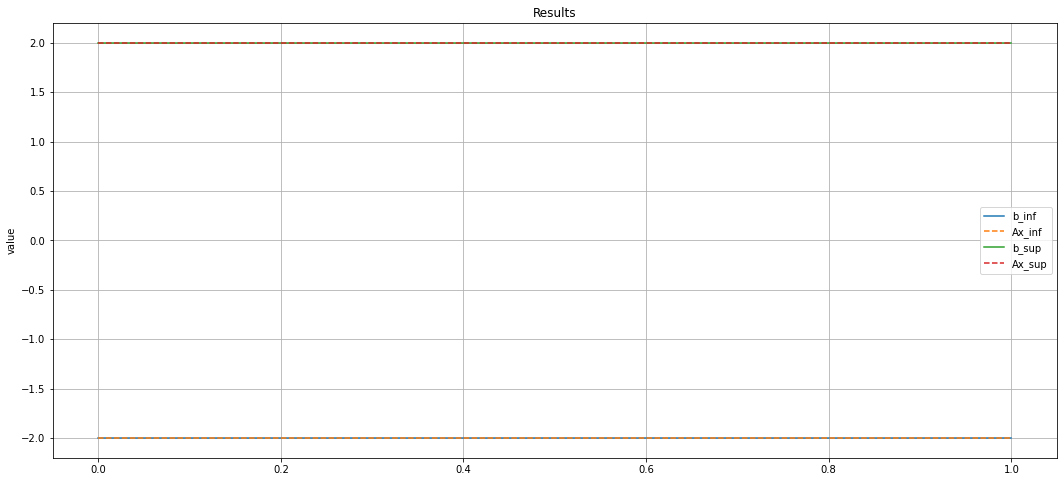
\includegraphics[width=10cm, height=6cm]{3.png}
        \caption{Результаты}
    \end{figure}
    
    
    \subsubsection{Треугольное расщепление}
    С помощью теоремы из пункта 2.2.2 получили, что метод треугольного расщепления матрицы на данной системе сходиться за конечное число итераций.
    
    Дейстивтельно, алгоритм сошелся за 11 итерации к следующим значениям 
    \begin{equation*}
        \begin{pmatrix}
             [-0.3333333, \ 0.3333333] \\
             [-0.3333332, \ 0.3333332] 
        \end{pmatrix}
    \end{equation*}
    Гарантируемая точность - 6 знаков после запятой.
     \begin{figure}[H]
        \centering
        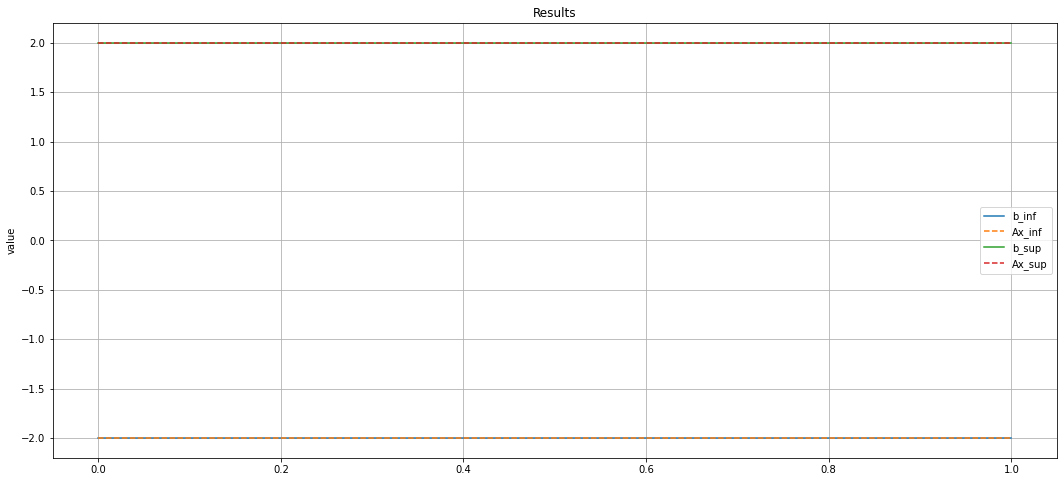
\includegraphics[width=10cm, height=6cm]{4.png}
        \caption{Результаты}
    \end{figure}
    
    
    \subsection{Решение поставленной задачи}
    Дана следующая ИСЛАУ 
    \begin{equation*}
        \begin{pmatrix}
             [4, \ 6] & [-9, \ 0] & [0, \ 12] & [2, \ 3] & [5, \ 9] & [-23, \ -9] & [15, \ 23]\\
             [0, \ 1] & [6, \ 10] & [-1, \ 1] & [-1, \ 3] & [-5, \ 1] & [1, \ 15] & [-3, \ -1]\\
             [0, \ 3] & [-20, \ -9] & [12, \ 77] & [-6, \ 30] & [0, \ 3] & [-18, \ 1] & [0, \ 1]\\
             [-4, \ 1] & [-1, \ 1] & [-3, \ 1] & [3, \ 5] & [5, \ 9] & [1, \ 2] & [1, \ 4]\\
             [0, \ 3] & [0, \ 6] & [0, \ 20] & [-1, \ 5] & [8, \ 15] & [-6, \ 1] & [10, \ 17]\\
             [-7, \ -2] & [1, \ 2] & [7, \ 14] & [-3, \ 1] & [0, \ 2] & [3, \ 5] & [-2, \ 1]\\
             [-1, \ 5] & [-3, \ 2] & [0, \ 8] & [1, \ 11] & [-5, \ 10] & [2, \ 7] & [6, \ 82]\\
        \end{pmatrix}
        x
        =
        \begin{pmatrix}
             [-10, \ 95] \\
             [35, \ 14] \\
             [-6, \ 2] \\
             [30, \ 7] \\
             [4, \ 95] \\
             [-6, \ 46] \\
             [-2, \ 65] 
        \end{pmatrix}
        
    \end{equation*}
    
    С помощью теоремы из пункта 2.1 получили, что матрица \textbf{A} является особенной.
    
    
    \subsubsection{Субдифференциальный метод}
    С помощью теоремы из пункта 2.2.1 получили, что субдифференциальный метод на данной системе \textbf{не} сходиться за конечное число итераций.\\
    
    Однако, алгоритм сошелся за 8 итерации к следующим значениям 
    \begin{equation*}
        \begin{pmatrix}
             [ -1.2247431, \ 0.5054298] \\
             [ 18.2644433, \  -9.517504] \\
             [ -0.0281865, \ 1.1607552] \\
             [ 16.4076957, \ -14.455534] \\
             [ -1.3435652, \ 3.9882184] \\
             [ -3.5289385, \ 4.5434583] \\
             [  5.4308623, \ -0.6740083]
        \end{pmatrix}
    \end{equation*}
    Гарантируемая точность - 6 знаков после запятой.
    
    То, что метод сошелся, является очень интересным фактом. В книге \cite{litlink3} это явление названо "mysterious behavior of the subdifferential Newton method"
     \begin{figure}[H]
        \centering
        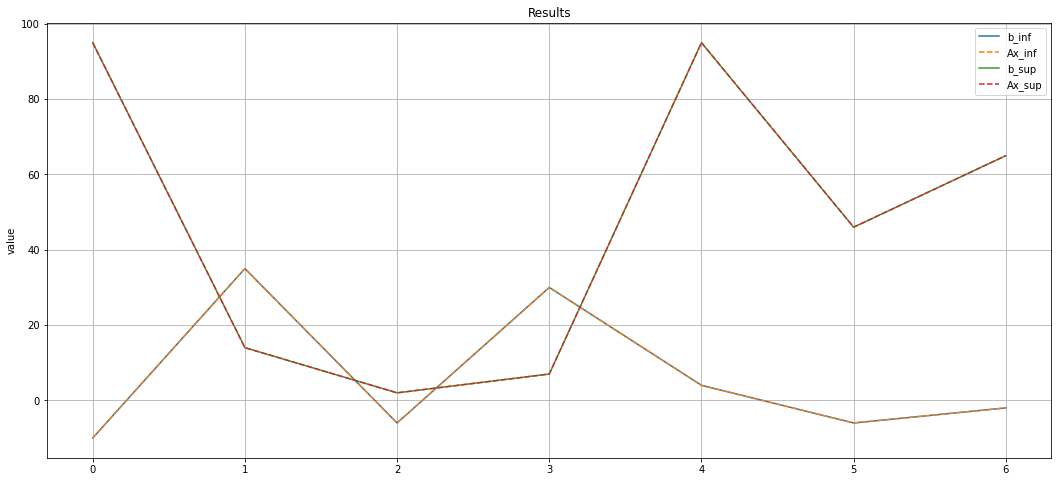
\includegraphics[width=10cm, height=6cm]{1.png}
        \caption{Результаты}
    \end{figure}
    
    
    \subsubsection{Треугольное расщепление}
    С помощью теоремы из пункта 2.2.2 получили, что метод треугольного расщепления матрицы на данной системе \textbf{не} сходиться за конечное число итераций.
    
    И дейстивтельно, алгоритм не сошелся за 100 итераций, а значения стремятся в бесконечность.
    \begin{figure}[H]
        \centering
        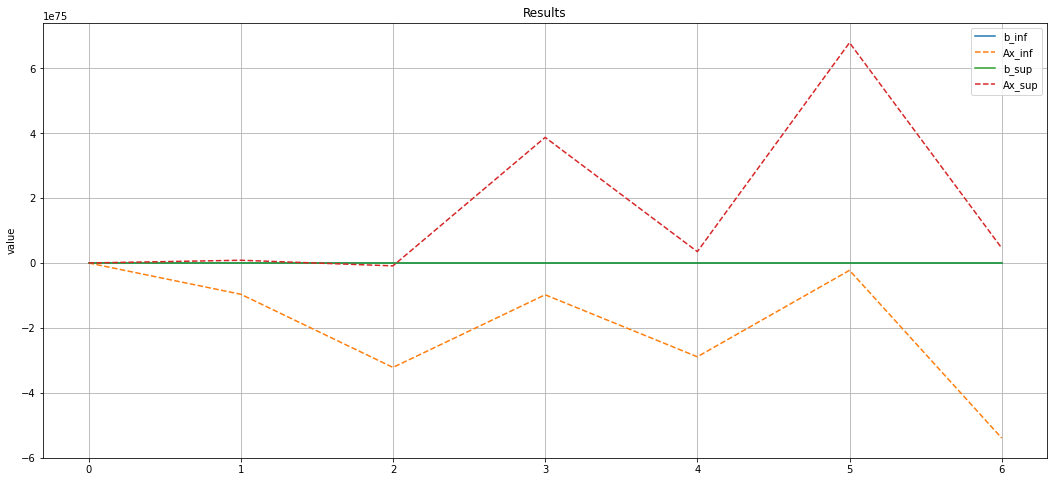
\includegraphics[width=10cm, height=6cm]{2.png}
        \caption{Результаты}
    \end{figure}
    
    \subsection{Эксперименты}
    \subsubsection{Субдифференциальный метод}
        Исследуем сходимость алгоритма, меняя один из элементов матрицы $\textbf{A}$. Будем менять нижнюю границу $\textbf{A}_{77}$
    \begin{table}[H]
			\centering
			\begin{tabular}{|c|c|}
				\hline
				$\textbf{A}_{77}$ & Результат\\
				
				\hline
				$[6, \ 82]$ & Сошелся \\
				
				\hline
				$[6.5, \ 82]$ & Сошелся \\
				
				\hline
				$[7, \ 82]$ & Сошелся \\
				
				\hline
				$[7.5, \ 82]$ & Сошелся \\
				
				\hline
				$[8, \ 82]$ & Не сошелся \\
				
				\hline
				$[8.5, \ 82]$ & Не сошелся \\
				
				\hline
				$[9, \ 82]$ & Не сошелся \\
				
				\hline
				$[9.5, \ 82]$ & Не сошелся \\
				
				\hline
				$[10, \ 82]$ & Не сошелся \\
				
				\hline
				$[10.5, \ 82]$ & Не сошелся \\
				
				\hline
				$[11, \ 82]$ & Сошелся \\
				
				\hline
				$[11.5, \ 82]$ & Сошелся \\
				
				\hline
				$[12, \ 82]$ & Сошелся \\
				
				\hline
				$[12.5, \ 82]$ & Сошелся \\

				\hline
				
			\end{tabular}
			\caption{Результаты при $\tau$=1}
		\end{table}
    
        Так же мы можем поменять релаксационный параметр данного алгоритма. Возьмем $\tau = 0.8$
        
        
            \begin{table}[H]
			\centering
			\begin{tabular}{|c|c|}
				\hline
				$\textbf{A}_{77}$ & Результат\\
				
				\hline
				$[6, \ 82]$ & Сошелся \\
				
				\hline
				$[6.5, \ 82]$ & Сошелся \\
				
				\hline
				$[7, \ 82]$ & Сошелся \\
				
				\hline
				$[7.5, \ 82]$ & Сошелся \\
				
				\hline
				$[8, \ 82]$ & Сошелся \\
				
				\hline
				$[8.5, \ 82]$ & Сошелся \\
				
				\hline
				$[9, \ 82]$ & Сошелся \\
				
				\hline
				$[9.5, \ 82]$ & Сошелся \\
				
				\hline
				$[10, \ 82]$ & Сошелся \\
				
				\hline
				$[10.5, \ 82]$ & Сошелся \\
				
				\hline
				$[11, \ 82]$ & Сошелся \\
				
				\hline
				$[11.5, \ 82]$ & Сошелся \\
				
				\hline
				$[12, \ 82]$ & Сошелся \\
				
				\hline
				$[12.5, \ 82]$ & Сошелся \\

				\hline
				
			\end{tabular}
			\caption{Результаты при $\tau$=0.8}
		\end{table}
		
		Поменяв параметр релаксации мы добились сходимости алгоритма на всех исследуемых значениях.
		
	    \subsubsection{Трегольное расщепление матрицы}
	    Проведем аналогичное изменение элемента $\textbf{A}_{77}$
	    
    \begin{table}[H]
			\centering
			\begin{tabular}{|c|c|}
				\hline
				$\textbf{A}_{77}$ & Результат\\
				
				\hline
				$[6, \ 82]$ & Не сошелся \\
				
				\hline
				$[6.5, \ 82]$ & Не сошелся \\
				
				\hline
				$[7, \ 82]$ & Не сошелся \\
				
				\hline
				$[7.5, \ 82]$ & Не сошелся \\
				
				\hline
				$[8, \ 82]$ & Не сошелся \\
				
				\hline
				$[8.5, \ 82]$ & Не сошелся \\
				
				\hline
				$[9, \ 82]$ & Не сошелся \\
				
				\hline
				$[9.5, \ 82]$ & Не сошелся \\
				
				\hline
				$[10, \ 82]$ & Не сошелся \\
				
				\hline
				$[10.5, \ 82]$ & Не сошелся \\
				
				\hline
				$[11, \ 82]$ & Не сошелся \\
				
				\hline
				$[11.5, \ 82]$ & Не сошелся \\
				
				\hline
				$[12, \ 82]$ & Не сошелся \\
				
				\hline
				$[12.5, \ 82]$ & Не сошелся \\

				\hline
				
			\end{tabular}
			\caption{Результаты при $\tau$=1}
		\end{table}
	    
	    Метод треугольного расщепления матрицы не сходиться нигде с требуемой точностью.
	    
    \subsection{Обсуждение}
    Можно сделать вывод, что субдифференциальный метод сходится за меньшее количество итераций, чем метод треугольного расщепления матрицы, с одинаковой точностью. Так же мы столкнулись с интересной осбоенностью субдифференциального метода - сходимость на некоторых особенных матрицах, что, несомненно, является его преимуществом. Так же субдифференциальный метод поддается настройке, что может значительно улучшить его свойства.
    
     
    
\newpage

\section{Приложения}
    \begin{itemize}
        \item Репозиторий с исходным кодом: \url{https://github.com/mitenevav/computer_complex/tree/master/course_project}
    \end{itemize}
   
\vspace{4cm} 
    
\addcontentsline{toc}{section}{Список используемой литературы}
 
%далее сам список используевой литературы
\begin{thebibliography}{}
    \bibitem{litlink1}  Баженов А. Н.  -  Интервальный анализ. Основы теории и учебные примеры: учебное пособие.  \url{https://elib.spbstu.ru/dl/2/s20-76.pdf/info}
    \bibitem{litlink2}  Шарый С. П.  -  Конечномерный интервальный анализ.
    \bibitem{litlink3}  Шарый С. П.  -  Алгебраический подход к интервальным линейным статическим задачам идентификации, о допусках и об управлении, или еще одно применение арифметики Каухера.
\end{thebibliography}

\end{document}
